\section{Pregled}

\subsection{Arhitektura}
Cijeli sustav je rastavljen u 3 glavna dijela
\begin{itemize}
  \item Transkoder
  \item Poslužitelj
  \item Klijenti
\end{itemize}
\paragraph{Transkoder}
je zadužen za primanje podataka od kamere i transformiranje istih u format koji je odgovarajuć za najveći broj klijenata, 
te slanje u realnom vremenu na poslužitelj putem TCP-a.
\paragraph{Poslužitelj}
je zadužen za autentifikaciju klijenata te prosljeđivanje paketa koje prima od Transkodera putem HTTP-a.
\paragraph{Klijenti}
nakon što se autoriziraju s poslužiteljom, primaju pakete videa putem HTTP-a te ih prikazuju korisniku.
\begin{figure}[h]
  \centering
  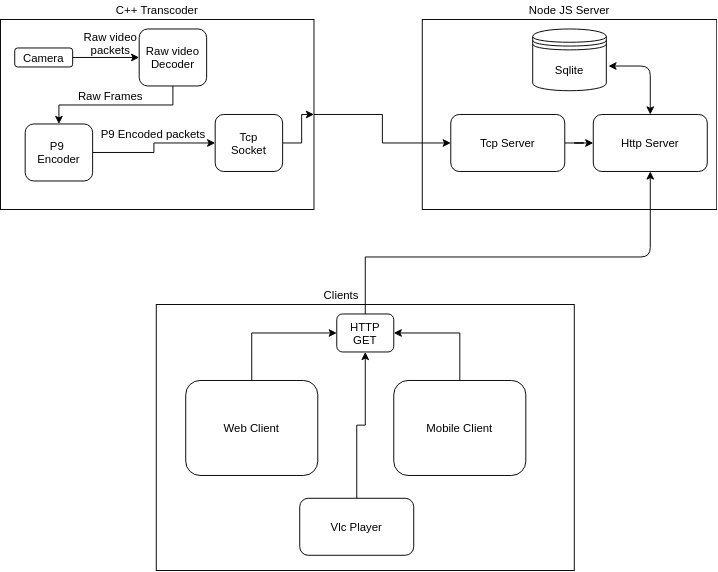
\includegraphics[height=10cm, width=\textwidth]{flow-diagram.png}
  \caption{Flow diagram sustava}
\end{figure}

\clearpage
\subsection{Tehnologije}

\subsubsection{C++}
C++ je odabran za implementaciju transkodera, primarno zato što su FFMpeg biblioteke napisane u jeziku C 
s kojim se C++ vrlo jednostavno integrira ali i zbog manjka memorije Raspberry pi-a i teške prirode posla kojeg obavlja
u smislu potrebne snage procesora zbog čega je bitno imati jezik koji se prevodi u nativni kod ovisno o platformi te koji
je memorijski učinkovit. \cite{bStrou}

\subsubsection{Node JS}
Node JS je \foreign{open-source cross-platform runtime} za JavaScript. \\
Omogućuje pisanje poslužiteljskog koda u jeziku JavaScript. \cite{nodeBook}
\paraBreak
Idealan je za poslužitelja ovog projekta zbog svog \foreign{event-driven} asinkronog pristupa.
Priroda posla koju poslužitelj obavlja ne zahtijeva veliku procesnu snagu nego mogućnost serviranja velikog broja zahtjeva
paralelno, \foreign{Node JS} se upravo u takvom tipu posla ističe. \cite{nodeBook}

\subsubsection{React JS}
React JS je \foreign{open-source} JavaScript biblioteka za izradu web aplikacija.
\paraBreak
Izabran je za implementaciju primjera web klijenta jer je klijent zamišljen da bude dinamična web aplikacija a ne statička
stranica, s potencijalno velikim brojem odlika. \cite{reactBook}
\paraBreak

\clearpage
\subsection{Video} \label{sec:video}
Video je ništa drugo nego niz slika koje se mijenjaju određenom frekvencijom, u slučaju filmova naj češće 24 slika 
po sekundi (24 FPS). \cite{ffmpegBook}

\subsubsection{Slika} \label{sec:slika}
Slika opisuje dekodirane čiste podatke videa. \\
U kontekstu enkodiranja postoje 3 glavne vrste \begin{itemize}
  \item \textbf{I} Slika - kompletna slika
  \item \textbf{P} Slika - predviđena slika, sadrži samo promjene od prethodne slike
  \item \textbf{B} Slika - slično kao i P, sadrži samo promjene ali ne samo od prethodne nego potencijalno i sljedeće 
  slike, te tako sačuva još više mjesta
\end{itemize}

\myparagraph{P i B Slike}
\foreign{P} i \foreign{B} slike su jedan od načina kojim enkoderi smanjuju finalnu veličinu datoteke, 
primjerice zamislimo kameru koja snima promet po noći,
većina slika tog videa će biti jako slična sve dok se ne pojavi auto, enkoder zato ne mora sve informacije spremati u svaku P sliku
već samo onaj dio slike gdje se pojavio auto dok ostatak uzme iz prethodne.
\paraBreak
To funkcionira tako da se uzme proizvoljan interval \foreign{I} slika, još poznatim kao \foreign{keyframe} recimo 
svakih 15 slika, tada enkoder svaku 15-tu sliku enkodira u potpunosti dok ostale enkodira kao \foreign{P} ili \foreign{B} slike.
\\
Što je interval I slika veći to će video u konačnici biti manji.
\paraBreak
Bitno je za znati da se na \foreign{P} i \foreign{B} slike ne može tražiti (\foreign{seek}), jer te slike sadrže samo frakciju podataka potrebnih
da se izgradi kompletna slika, recimo da imamo video koji se vrti 30 slika u sekundi te enkodiramo \foreign{I} sliku 
svakih 10 sekundi ili 900 slika, tada bi video bilo moguće premotavati naprijed ili nazad samo u intervalima od 10 sekundi.
\paraBreak
Stoga ako je bitno da se video može premotavati u malim intervalima mora se postaviti Interval \foreign{I} 
slika na što manju vrijednost.

\subsubsection{Piksel format} \label{sec:pixelformat}
Piksel format je format ili način na koji je svaki pojedinačni piksel slike zapisan odnosno opisuje kako su podaci o boji
svakog piksela enkodirani. Primjerice piksel format \foreign{24 bit RGB} još poznat kao \foreign{RGB888} 
zauzima 3 bajta po pikselu, jedan bajt za svaki od kanala.
\paraBreak
Enkoderi preferiraju \textbf{planarne} piksel formate, primjerice h264 enkoder podržava samo \foreign{yuv420p} piksel format, što
znači da se za enkodiranje tipičnog videa mora raditi pretvorba iz RGB piksel formata u yuv420p. \\
Jedan od razloga je memorijska efikasnost, primjerice \foreign{RGB888} piksel format zauzima 3 bajta po pikselu dok
yuv420p zauzima 6 bajta svaka 4 piksela. \cite{ffmpegBook}

\paragraph{Planaran} \label{sec:planar} piksel format znaci da predstavlja boje piksela kroz nekoliko ravnina ili 
ploha, uglavnom 3 ravnine. \\
Svaki bit ovih ravnina predstavlja dio piksela slike. To je korisno jer se podaci o pikselu više ne nalaze u jednom 
neprekidnom polju odnosno istoj lokaciji u memoriji, nego su razdvojeni na više polja.

\subsubsection{Kontejner} \label{sec:container}
Kontejner je jedna datoteka koja sadrži sve tokove kao što su video, audio i titlovi.\\
Još sadrži sve metapodatke kao što su rezolucija videa, FPS, autor, kodek itd. Po tim 
podacima \hyperref[sct:videoPlayer]{\foreign{video player}}-i znaju korektno prikazati sliku i zvuk. \cite{ffmpegBook}
\\
Primjeri nekih kontejnera su:
\begin{itemize}
  \item MPEG-4
  \item Matroska
  \item QuickTime/MP4
  \item WebM
  \item WAW
\end{itemize}

\subsubsection{Kodek} \label{sec:codec}
Kodek je softver (ili hardver) koji služi za kompresiju ili dekompresiju videa. \\
Pretvara ne kompresiran (\foreign{Raw}) video u kompresiran i obratno. \\
Ako je riječ o kompresiranju onda je to enkoder, inače dekoder. \cite{ffmpegBook}
\paraBreak
Proces kompresiranja je tipično gubitačan (\foreign{lossy}) što znači da kompresirani video ne sadrži sve informacije kao i original
što rezultira u lošijoj kvaliteti videa i nakon kompresije više nije moguće u potpunosti rekonstruirati original. \cite{ffmpegBook}
\paraBreak
Problem kod videa je veličina, recimo da imamo video rezolucije 1920 x 1080 koji se vrti na 24 slika u sekundi, i da 
koristimo RGB piksel format što znači da nam trebaju 3 bajta po pikselu za enkodiranje boje te da traje 30 minuta 
(trećina ili manje prosječnog filma) \\
Veličina takvog videa bez enkodiranja bila bi \textbf{268.7 GB} \label{sec:size_problem} \cite{ffmpegBook}
\paraBreak
Upravo iz tog razloga moramo imati kodek.

\subsubsection{Podržanost}
Za živi prijenos postoje 3 naj bolje opcije što se tiče podržanosti \cite{appleCodec} \cite{androidCodec} \cite{canIUse}

\begin{center}
  \begin{table}[h]
    \begin{tabular}{|c|c|c|c|}
      \hline
      & vp8/9 + webm & h264+mp4/DASH & h264 + mkv \\
      \hline
      Chrome & x & x & - \\
      Firefox & x & x & - \\
      Safari & - & x & - \\
      Edge & vp8 & x & - \\
      IOS (Svi preglednici) & - & x & - \\
      Android (Chrome) & x & x & - \\
      \hline
    \end{tabular}
    \caption[Podržanost kodeka i kontejnera u raznim preglednicima]
    {Podržanost kodeka i kontejnera u raznim preglednicima \cite{appleCodec} \cite{androidCodec} \cite{canIUse}}
\end{table}

\end{center}

\myparagraph{h264 + rtmp}
H264 je jedan od starijih kodeka i kao takav podržan je na skoro svim uređajima.
Nudi dobar balans kvalitete i brzine. \cite{h264Book}
\paraBreak
Rtmp kontejner je jedan od naj korištenijih kontejnera za živi prijenos, jedan od korisnika je Twitch.tv \\
Problem ovog kontejnera je sto je vlasnik Adobe i nije besplatan, uz to nije podržan nativno u HTML5 video elementu.

\myparagraph{h264 + mp4}
U teoriji odlična kombinacija jer je mp4 kontejner podržan virtualno svugdje.
\paraBreak
Nažalost mp4 ne podržava živi prijenos jer mora unaprijed znati točnu duljinu videa što kod živog prijenosa nije moguće. \\
Rješenje je MPEG-DASH (Dynamic Adaptive Streaming over HTTP). Proces razdvajanja videa u manje cjeline s poznatom veličinom.

\myparagraph{vp8/9 + webm}
Ovu kombinaciju kodeka i kontejnera je implementirao Google, želeći izbjeći troškove licenci za 264/5 kodek. \\
Glavna snaga mu je odlična kompatibilnost s nativnim HTML 5 video elementom koji je standard u većini preglednika \cite{ffmpegBook}
\paraBreak
Osim toga u usporedbi s puno starijim h264 kodekom, pruža bolju latenciju i kvalitetu slike, pogotovo 
na nižim \hyperref[sct:bitRate]{\foreign{bit rate}} a uz to je i efikasniji što se tiče resursa. \cite{ffmpegBook}
\paraBreak
Najveći problem mu je Apple koji odbija implementirati ovu kombinaciju u Safariju i IOS operativnom sustavu. \\
Također za razliku od mp4 kontejnera webm nije kodek agnostičan, to jest može se kombinirati samo sa vp8 ili vp9 kodecima. \cite{ffmpegBook}
\paraBreak
Upravo ova kombinacija je odabrana u ovom radu zbog svoje relativne jednostavnosti i dobre podržanosti.
